\chapter{Introducción}

\section{Antecedentes}

\subsection{Historia y evolución de las JAAPS en Ecuador}
TODO

\subsection{Contexto de la gestión del agua en zonas rurales}
TODO

\subsection{Tecnologías actuales de medición de consumo de agua}
TODO

\section{Problemática}

\subsection{Descripción del proceso manual actual}
TODO

\subsection{Demoras operativas en la lectura de medidores}
TODO

\subsection{Problemas de conectividad en zonas rurales}
TODO

\subsection{Errores de digitación y su impacto económico}
TODO

\section{Justificación}

\subsection{Componente de investigación}

\subsubsection{Avances en visión por computadora móvil}
TODO

\subsubsection{Estado actual del OCR en dispositivos edge}
TODO

\subsubsection{Brechas identificadas en la literatura}
TODO

\subsection{Componente de innovación}

\subsubsection{Solución novedosa para contexto rural}
TODO

\subsubsection{Adaptación tecnológica a recursos limitados}
TODO

\subsubsection{Potencial de escalabilidad}
TODO

\subsection{Componente técnico}

\subsubsection{Viabilidad técnica demostrada}
TODO

\subsubsection{Tecnologías maduras disponibles}
TODO

\subsubsection{Capacidades actuales de dispositivos móviles}
TODO

\section{Objetivos}

\subsection{Objetivo general}
TODO

\subsection{Objetivos específicos}
TODO

\section{Estructura del documento}
TODO

\begin{table}[H]
\centering
\caption{Xxxxxxxx}
\label{tab:tabla1}
\begin{tabular}{@{}lcccc@{}}
\toprule
\multirow{2}{*}{\textbf{Internet}} & \multicolumn{2}{c}{\textbf{Urbano}} & \multicolumn{2}{c}{\textbf{Rural}} \\
\cmidrule(lr){2-3} \cmidrule(lr){4-5}
 & 06 a 09 & 10 a 11 & 06 a 09 & 10 a 11 \\
\midrule
Grado a & 10 & 15 & 2 & 4 \\
Grado b & 15 & 18 & 3 & 3 \\
Grado c & 15 & 10 & 3 & 1 \\
Grado d & 10 & 20 & 2 & 1 \\
\midrule
\textbf{Total} & 50 & 63 & 10 & 9 \\
\bottomrule
\end{tabular}
\vspace{0.5cm}\\
\textit{Nota}. Esta tabla se observa que los niños del sector urbano tienen mayor acceso al Internet.
\end{table}

\subsection{Xxxxxxxx xxxxxxxx xxxxxxxxxxx}

Xxxxxxxxxxxxxxxxxxxxxxxxxxxxxxxxxxxxxxxxxxxxxxxxxxxxxxxxxxxxxxxxxxxxxxxxxxxxxxxxxxxxxxxxxxxxxxx xxxxxxxxxxxxxx xxxxxxxx xxxxxxxxxxxxxxxxxxxxxxxxxxxxxxxxxxxx xxxxxxxxxxxx xxxxxxxxxxxxxxxxxxxxxx xxxxxxxxxxxxxxxxxxxxx.

\subsubsection{Xxxx xxxx xxxxxxx.} Xxxxxxxxxxxxxxxxxx xxxxx xxxxxx xxxxxxxxxxxxx xxxxxxxxxxxx.

\paragraph{Xxxx xxxxxxx xxx xxxx.} Xxxxxxxxxxxx xxxxxxxx xxxxxxxxxx xxxxxxx xxxxxxxxxxxx.

\begin{figure}[H]
\centering
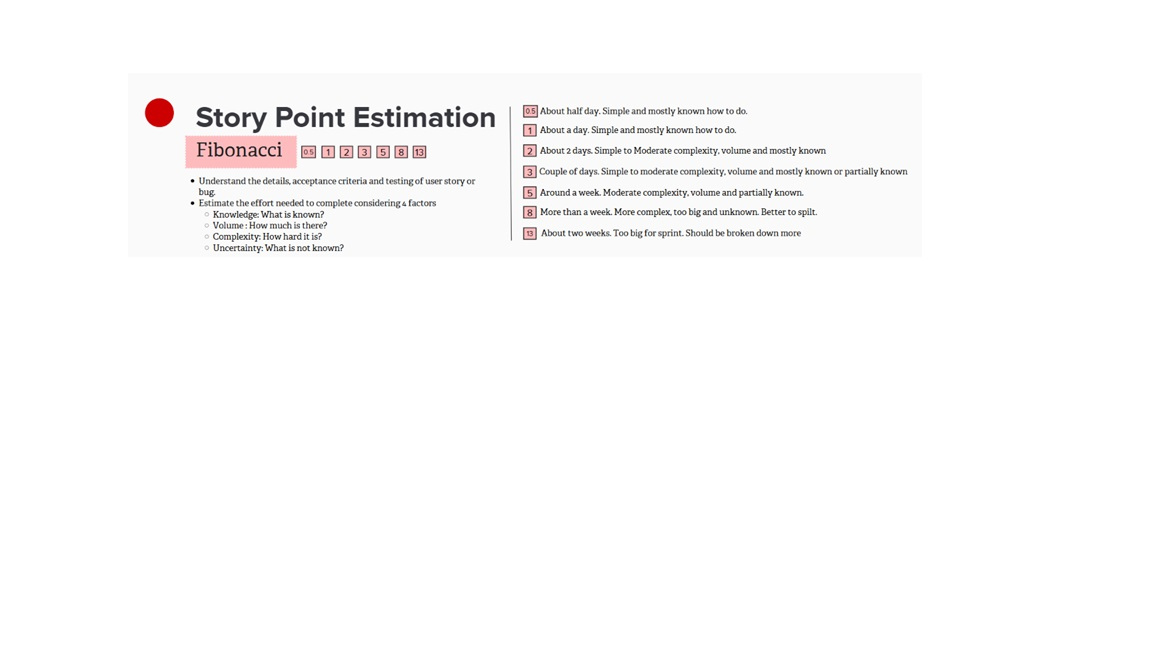
\includegraphics[width=0.7\textwidth]{figures/example.jpg}
\caption{Xxxxx}
\label{fig:figura1}
\textit{Nota}. Adaptado de Virus VIH [Fotografía], por Consejo Superior de Investigaciones Científicas, 2011, Flickr (flic.kr/p/aronSf). CC BY 2.0.
\end{figure}